\documentclass[10pt]{article}
\usepackage[polish]{babel}
\usepackage[utf8]{inputenc}
\usepackage[T1]{fontenc}
\usepackage{graphicx}
\usepackage[export]{adjustbox}
\graphicspath{ {./images/} }
\usepackage{amsmath}
\usepackage{amsfonts}
\usepackage{amssymb}
\usepackage[version=4]{mhchem}
\usepackage{stmaryrd}
\usepackage{multirow}

\title{EGZAMIN MATURALNY \\
 Z MATEMATYKI POZIOM PODSTAWOWY }

\author{Data: 7 maja 2018 r.\\
Godzina rozpoczecia: 9:00\\
CZaS PRACY: 170 minut}
\date{}


\begin{document}
\maketitle
\begin{center}
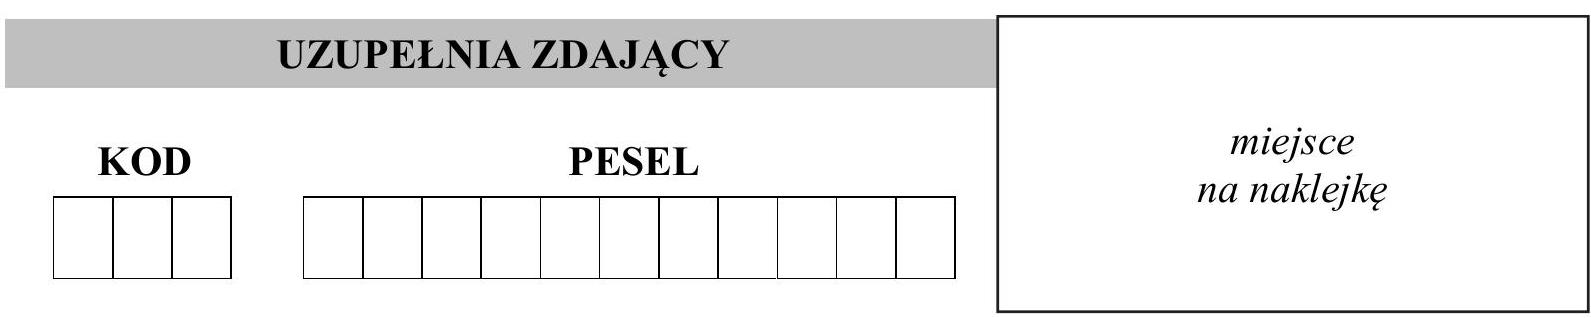
\includegraphics[max width=\textwidth]{2024_11_21_13fdaeec1d7100ca9ddcg-01(1)}
\end{center}

UZUPELNIA ZESPÓL NADZORUJĄCY\\
Uprawnienia zdającego do:

\(\square \quad\)\begin{tabular}{l}
dostosowania \\
kryteriów oceniania \\
\end{tabular}

\(\square \quad\)\begin{tabular}{l}
nieprzenoszenia \\
zaznaczén na kartę \\
\end{tabular}

\(\square \quad\)\begin{tabular}{l}
dostosowania \\
w zw. z dyskalkulią \\
\end{tabular}

LicZba PunKTów do UZYSKania: \(\mathbf{5 0}\)

\section*{Instrukcja dla zdającego}
\begin{enumerate}
  \item Sprawdź, czy arkusz egzaminacyjny zawiera 26 stron (zadania 1-34). Ewentualny brak zgłoś przewodniczącemu zespołu nadzorującego egzamin.
  \item Rozwiązania zadań i odpowiedzi wpisuj w miejscu na to przeznaczonym.
  \item Odpowiedzi do zadań zamkniętych (1-25) zaznacz na karcie odpowiedzi, w części karty przeznaczonej dla zdającego. Zamaluj \(\square\) pola do tego przeznaczone. Błędne zaznaczenie otocz kółkiem \(\bigcirc_{\text {i zaznacz właściwe. }}\)
  \item Pamiętaj, że pominięcie argumentacji lub istotnych obliczeń w rozwiązaniu zadania otwartego (26-34) może spowodować, że za to rozwiązanie nie otrzymasz pełnej liczby punktów.
  \item Pisz czytelnie i używaj tylko długopisu lub pióra z czarnym tuszem lub atramentem.
  \item Nie używaj korektora, a błędne zapisy wyraźnie przekreśl.\\

\includegraphics[max width=\textwidth, center]{2024_11_21_13fdaeec1d7100ca9ddcg-01(2)}
  \item Pamiętaj, że zapisy w brudnopisie nie będą oceniane.
  \item Możesz korzystać z zestawu wzorów matematycznych, cyrkla i linijki, a także z kalkulatora prostego.
  \item Na tej stronie oraz na karcie odpowiedzi wpisz swój numer PESEL i przyklej naklejkę z kodem.
  \item Nie wpisuj żadnych znaków w części przeznaczonej dla egzaminatora.\\

\includegraphics[max width=\textwidth, center]{2024_11_21_13fdaeec1d7100ca9ddcg-01}
\end{enumerate}

W każdym z zadań od 1. do 25. wybierz i zaznacz na karcie odpowiedzi poprawnq̨ odpowiedź.

\section*{Zadanie 1. (0-1)}
Liczba \(2 \log _{3} 6-\log _{3} 4\) jest równa\\
A. 4\\
B. 2\\
C. \(2 \log _{3} 2\)\\
D. \(\log _{3} 8\)

\section*{Zadanie 2. (0-1)}
Liczba \(\sqrt[3]{\frac{7}{3}} \cdot \sqrt[3]{\frac{81}{56}}\) jest równa\\
A. \(\frac{\sqrt{3}}{2}\)\\
B. \(\frac{3}{2 \sqrt[3]{21}}\)\\
C. \(\frac{3}{2}\)\\
D. \(\frac{9}{4}\)

\section*{Zadanie 3. (0-1)}
Dane są liczby \(a=3,6 \cdot 10^{-12}\) oraz \(b=2,4 \cdot 10^{-20}\). Wtedy iloraz \(\frac{a}{b}\) jest równy\\
A. \(8,64 \cdot 10^{-32}\)\\
B. \(1,5 \cdot 10^{-8}\)\\
C. \(1,5 \cdot 10^{8}\)\\
D. \(8,64 \cdot 10^{32}\)

\section*{Zadanie 4. (0-1)}
Cena roweru po obniżce o \(15 \%\) była równa 850 zł. Przed obniżką ten rower kosztował\\
A. \(865,00 \mathrm{zt}\)\\
B. \(850,15 \mathrm{zt}\)\\
C. \(1000,00 \mathrm{zł}\)\\
D. \(977,50 \mathrm{zt}\)

\section*{Zadanie 5. (0-1)}
Zbiorem wszystkich rozwiązań nierówności \(\frac{1-2 x}{2}>\frac{1}{3}\) jest przedział\\
A. \(\left(-\infty, \frac{1}{6}\right)\)\\
B. \(\left(-\infty, \frac{2}{3}\right)\)\\
C. \(\left(\frac{1}{6},+\infty\right)\)\\
D. \(\left(\frac{2}{3},+\infty\right)\)

\section*{Zadanie 6. (0-1)}
Funkcja kwadratowa jest określona wzorem \(f(x)=-2(x+3)(x-5)\). Liczby \(x_{1}, x_{2}\) są różnymi miejscami zerowymi funkcji \(f\). Zatem\\
A. \(x_{1}+x_{2}=-8\)\\
B. \(x_{1}+x_{2}=-2\)\\
C. \(x_{1}+x_{2}=2\)\\
D. \(x_{1}+x_{2}=8\)

\section*{BRUDNOPIS (nie podlega ocenie)}
\begin{center}
\begin{tabular}{|c|c|c|c|c|c|c|c|c|c|c|c|c|c|c|c|c|c|c|c|c|c|c|c|c|c|c|}
\hline
 &  &  &  &  &  &  &  &  &  &  &  &  &  &  &  &  &  &  &  &  &  &  &  &  &  &  \\
\hline
 &  &  &  &  &  &  &  &  &  &  &  &  &  &  &  &  &  &  &  &  &  &  &  &  &  &  \\
\hline
 &  &  &  &  &  &  &  &  &  &  &  &  &  &  &  &  &  &  &  &  &  &  &  &  &  &  \\
\hline
 &  &  &  &  &  &  &  &  &  &  &  &  &  &  &  &  &  &  &  &  &  &  &  &  &  &  \\
\hline
 &  &  &  &  &  &  &  &  &  &  &  &  &  &  &  &  &  &  &  &  &  &  &  &  &  &  \\
\hline
 &  &  &  &  &  &  &  &  &  &  &  &  &  &  &  &  &  &  &  &  &  &  &  &  &  &  \\
\hline
 &  &  &  &  &  &  &  &  &  &  &  &  &  &  &  &  &  &  &  &  &  &  &  &  &  &  \\
\hline
 &  &  &  &  &  &  &  &  &  &  &  &  &  &  &  &  &  &  &  &  &  &  &  &  &  &  \\
\hline
 &  &  &  &  &  &  &  &  &  &  &  &  &  &  &  &  &  &  &  &  &  &  &  &  &  &  \\
\hline
 &  &  &  &  &  &  &  &  &  &  &  &  &  &  &  &  &  &  &  &  &  &  &  &  &  &  \\
\hline
 &  &  &  &  &  &  &  &  &  &  &  &  &  &  &  &  &  &  &  &  &  &  &  &  &  &  \\
\hline
 &  &  &  &  &  &  &  &  &  &  &  &  &  &  &  &  &  &  &  &  &  &  &  &  &  &  \\
\hline
 &  &  &  &  &  &  &  &  &  &  &  &  &  &  &  &  &  &  &  &  &  &  &  &  &  &  \\
\hline
 &  &  &  &  &  &  &  &  &  &  &  &  &  &  &  &  &  &  &  &  &  &  &  &  &  &  \\
\hline
 &  &  &  &  &  &  &  &  &  &  &  &  &  &  &  &  &  &  &  &  &  &  &  &  &  &  \\
\hline
 &  &  &  &  &  &  &  &  &  &  &  &  &  &  &  &  &  &  &  &  &  &  &  &  &  &  \\
\hline
 &  &  &  &  &  &  &  &  &  &  &  &  &  &  &  &  &  &  &  &  &  &  &  &  &  &  \\
\hline
 &  &  &  &  &  &  &  &  &  &  &  &  &  &  &  &  &  &  &  &  &  &  &  &  &  &  \\
\hline
 &  &  &  &  &  &  &  &  &  &  &  &  &  &  &  &  &  &  &  &  &  &  &  &  &  &  \\
\hline
 &  &  &  &  &  &  &  &  &  &  &  &  &  &  &  &  &  &  &  &  &  &  &  &  &  &  \\
\hline
 &  &  &  &  &  &  &  &  &  &  &  &  &  &  &  &  &  &  &  &  &  &  &  &  &  &  \\
\hline
 &  &  &  &  &  &  &  &  &  &  &  &  &  &  &  &  &  &  &  &  &  &  &  &  &  &  \\
\hline
 &  &  &  &  &  &  &  &  &  &  &  &  &  &  &  &  &  &  &  &  &  &  &  &  &  &  \\
\hline
 &  &  &  &  &  &  &  &  &  &  &  &  &  &  &  &  &  &  &  &  &  &  &  &  &  &  \\
\hline
 &  &  &  &  &  &  &  &  &  &  &  &  &  &  &  &  &  &  &  &  &  &  &  &  &  &  \\
\hline
 &  &  &  &  &  &  &  &  &  &  &  &  &  &  &  &  &  &  &  &  &  &  &  &  &  &  \\
\hline
 &  &  &  &  &  &  &  & 
\includegraphics[max width=\textwidth]{2024_11_21_13fdaeec1d7100ca9ddcg-03}
 &  &  &  &  &  &  &  &  &  &  &  &  &  &  &  &  &  &  \\
\hline
 &  &  &  &  &  &  &  &  &  &  &  &  &  &  &  &  &  &  &  &  &  &  &  &  &  &  \\
\hline
 &  &  &  &  &  &  &  &  &  &  &  &  &  &  &  &  &  &  &  &  &  &  &  &  &  &  \\
\hline
 &  &  &  &  &  &  &  &  &  &  &  &  &  &  &  &  &  &  &  &  &  &  &  &  &  &  \\
\hline
 &  &  &  &  &  &  &  &  &  &  &  &  &  &  &  &  &  &  &  &  &  &  &  &  &  &  \\
\hline
 &  &  &  &  &  &  &  &  &  &  &  &  &  &  &  &  &  &  &  &  &  &  &  &  &  &  \\
\hline
 &  &  &  &  &  &  &  &  &  &  &  &  &  &  &  &  &  &  &  &  &  &  &  &  &  &  \\
\hline
 &  &  &  &  &  &  &  &  &  &  &  &  &  &  &  &  &  &  &  &  &  &  &  &  &  &  \\
\hline
 &  &  &  &  &  &  &  &  &  &  &  &  &  &  &  &  &  &  &  &  &  &  &  &  &  &  \\
\hline
 & \textbackslash  &  &  &  &  &  &  &  &  &  &  &  &  &  &  &  &  &  &  &  &  &  &  &  &  &  \\
\hline
 & - &  &  &  &  &  &  &  &  &  &  &  &  &  &  &  &  &  &  &  &  &  &  &  &  &  \\
\hline
 & - &  &  &  &  &  &  &  &  &  &  &  &  &  &  &  &  &  &  &  &  &  &  &  &  &  \\
\hline
 & \textbackslash  &  &  &  &  &  &  &  &  &  &  &  &  &  &  &  &  &  &  &  &  &  &  &  &  &  \\
\hline
 & \(\square\) &  &  &  &  &  &  &  &  &  &  &  &  &  &  &  &  &  &  &  &  &  &  &  &  &  \\
\hline
 &  &  &  &  &  &  &  &  &  &  &  &  &  &  &  &  &  &  &  &  &  &  &  &  &  &  \\
\hline
 & \textbackslash  &  &  &  &  &  &  &  &  &  &  &  &  &  &  &  &  &  &  &  &  &  &  &  &  &  \\
\hline
 &  &  &  &  &  &  &  &  &  &  &  &  &  &  &  &  &  &  &  &  &  &  &  &  &  &  \\
\hline
 &  &  &  &  &  &  &  &  &  &  &  &  &  &  &  &  &  &  &  &  &  &  &  &  &  &  \\
\hline
 & , &  &  &  &  &  &  &  &  &  &  &  &  &  &  &  &  &  &  &  &  &  &  &  &  &  \\
\hline
 &  &  &  &  &  &  &  &  &  &  &  &  &  &  &  &  &  &  &  &  &  &  &  &  &  &  \\
\hline
 &  &  &  & 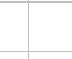
\includegraphics[max width=\textwidth]{2024_11_21_13fdaeec1d7100ca9ddcg-03(1)}
 &  &  &  &  &  &  &  &  &  &  &  &  &  &  &  &  &  &  &  &  &  &  \\
\hline
 &  &  &  &  &  &  &  &  &  &  &  &  &  &  &  &  &  &  &  &  &  &  &  &  &  &  \\
\hline
\end{tabular}
\end{center}

\section*{Zadanie 7. (0-1)}
Równanie \(\frac{x^{2}+2 x}{x^{2}-4}=0\)\\
A. ma trzy rozwiązania: \(x=-2, x=0, x=2\)\\
B. ma dwa rozwiązania: \(x=0, x=-2\)\\
C. ma dwa rozwiązania: \(x=-2, x=2\)\\
D. ma jedno rozwiązanie: \(x=0\)

\section*{Zadanie 8. (0-1)}
Funkcja liniowa \(f\) określona jest wzorem \(f(x)=\frac{1}{3} x-1\), dla wszystkich liczb rzeczywistych \(x\). Wskaż zdanie prawdziwe.\\
A. Funkcja \(f\) jest malejąca i jej wykres przecina oś \(O y\) w punkcie \(P=\left(0, \frac{1}{3}\right)\).\\
B. Funkcja \(f\) jest malejąca i jej wykres przecina oś \(O y\) w punkcie \(P=(0,-1)\).\\
C. Funkcja \(f\) jest rosnąca i jej wykres przecina oś \(O y\) w punkcie \(P=\left(0, \frac{1}{3}\right)\).\\
D. Funkcja \(f\) jest rosnąca i jej wykres przecina oś \(O y\) w punkcie \(P=(0,-1)\).

\section*{Zadanie 9. (0-1)}
Wykresem funkcji kwadratowej \(f(x)=x^{2}-6 x-3\) jest parabola, której wierzchołkiem jest punkt o współrzędnych\\
A. \((-6,-3)\)\\
B. \((-6,69)\)\\
C. \((3,-12)\)\\
D. \((6,-3)\)

\section*{Zadanie 10. (0-1)}
Liczba 1 jest miejscem zerowym funkcji liniowej \(f(x)=a x+b\), a punkt \(M=(3,-2)\) należy do wykresu tej funkcji. Współczynnik \(a\) we wzorze tej funkcji jest równy\\
A. 1\\
B. \(\frac{3}{2}\)\\
C. \(-\frac{3}{2}\)\\
D. -1

\section*{Zadanie 11. (0-1)}
Dany jest ciąg \(\left(a_{n}\right)\) określony wzorem \(a_{n}=\frac{5-2 n}{6}\) dla \(n \geq 1\). Caąg ten jest\\
A. arytmetyczny i jego różnica jest równa \(r=-\frac{1}{3}\).\\
B. arytmetyczny i jego różnica jest równa \(r=-2\).\\
C. geometryczny i jego iloraz jest równy \(q=-\frac{1}{3}\).\\
D. geometryczny i jego iloraz jest równy \(q=\frac{5}{6}\).

\section*{BRUDNOPIS (nie podlega ocenie)}
\begin{center}
\begin{tabular}{|c|c|c|c|c|c|c|c|c|c|c|c|c|c|c|c|c|c|c|c|c|c|c|c|c|c|c|}
\hline
 &  &  &  &  &  &  &  &  &  &  &  &  &  &  &  &  &  &  &  &  &  &  &  &  &  &  \\
\hline
 &  &  &  &  &  &  &  &  &  &  &  &  &  &  &  &  &  &  &  &  &  &  &  &  &  &  \\
\hline
 &  &  &  &  &  &  &  &  &  &  &  &  &  &  &  &  &  &  &  &  &  &  &  &  &  &  \\
\hline
 &  &  &  &  &  &  &  &  &  &  &  &  &  &  &  &  &  &  &  &  &  &  &  &  &  &  \\
\hline
 &  &  &  &  &  &  &  &  &  &  &  &  &  &  &  &  &  &  &  &  &  &  &  &  &  &  \\
\hline
 &  &  &  &  &  &  &  &  &  &  &  &  &  &  &  &  &  &  &  &  &  &  &  &  &  &  \\
\hline
 &  &  &  &  &  &  &  &  &  &  &  &  &  &  &  &  &  &  &  &  &  &  &  &  &  &  \\
\hline
 &  &  &  &  &  &  &  &  &  &  &  &  &  &  &  &  &  &  &  &  &  &  &  &  &  &  \\
\hline
 &  &  &  &  &  &  &  &  &  &  &  &  &  &  &  &  &  &  &  &  &  &  &  &  &  &  \\
\hline
 &  &  &  &  &  &  &  &  &  &  &  &  &  &  &  &  &  &  &  &  &  &  &  &  &  &  \\
\hline
 &  &  &  &  &  &  &  &  &  &  &  &  &  &  &  &  &  &  &  &  &  &  &  &  &  &  \\
\hline
 &  &  &  &  &  &  &  &  &  &  &  &  &  &  &  &  &  &  &  &  &  &  &  &  &  &  \\
\hline
 &  &  &  &  &  &  &  &  &  &  &  &  &  &  &  &  &  &  &  &  &  &  &  &  &  &  \\
\hline
 &  &  &  &  &  &  &  &  &  &  &  &  &  &  &  &  &  &  &  &  &  &  &  &  &  &  \\
\hline
 &  &  &  &  &  &  &  &  &  &  &  &  &  &  &  &  &  &  &  &  &  &  &  &  &  &  \\
\hline
 &  &  &  &  &  &  &  &  &  &  &  &  &  &  &  &  &  &  &  &  &  &  &  &  &  &  \\
\hline
 &  &  &  &  &  &  &  &  &  &  &  &  &  &  &  &  &  &  &  &  &  &  &  &  &  &  \\
\hline
 &  &  &  &  &  &  &  &  &  &  &  &  &  &  &  &  &  &  &  &  &  &  &  &  &  &  \\
\hline
 &  &  &  &  &  &  &  &  &  &  &  &  &  &  &  &  &  &  &  &  &  &  &  &  &  &  \\
\hline
 &  &  &  &  &  &  &  &  &  &  &  &  &  &  &  &  &  &  &  &  &  &  &  &  &  &  \\
\hline
 &  &  &  &  &  &  &  &  &  &  &  &  &  &  &  &  &  &  &  &  &  &  &  &  &  &  \\
\hline
 &  &  &  &  &  &  &  &  &  &  &  &  &  &  &  &  &  &  &  &  &  &  &  &  &  &  \\
\hline
 &  &  &  &  &  &  &  &  &  &  &  &  &  &  &  &  &  &  &  &  &  &  &  &  &  &  \\
\hline
 &  &  &  &  &  &  &  &  &  &  &  &  &  &  &  &  &  &  &  &  &  &  &  &  &  &  \\
\hline
 &  &  &  &  &  &  &  &  &  &  &  &  &  &  &  &  &  &  &  &  &  &  &  &  &  &  \\
\hline
 &  &  &  &  &  &  &  &  &  &  &  &  &  &  &  &  &  &  &  &  &  &  &  &  &  &  \\
\hline
 &  &  &  &  &  &  &  & 
\includegraphics[max width=\textwidth]{2024_11_21_13fdaeec1d7100ca9ddcg-05}
 &  & 
\includegraphics[max width=\textwidth]{2024_11_21_13fdaeec1d7100ca9ddcg-05(1)}
 &  &  &  &  &  &  &  &  &  &  &  &  &  &  &  &  \\
\hline
 &  &  &  &  &  &  &  &  &  &  &  &  &  &  &  &  &  &  &  &  &  &  &  &  &  &  \\
\hline
 &  &  &  &  &  &  &  &  &  &  &  &  &  &  &  &  &  &  &  &  &  &  &  &  &  &  \\
\hline
 &  &  &  &  &  &  &  &  &  &  &  &  &  &  &  &  &  &  &  &  &  &  &  &  &  &  \\
\hline
 &  &  &  &  &  &  &  &  &  &  &  &  &  &  &  &  &  &  &  &  &  &  &  &  &  &  \\
\hline
 &  &  &  &  &  &  &  &  &  &  &  &  &  &  &  &  &  &  &  &  &  &  &  &  &  &  \\
\hline
 &  &  &  &  &  &  &  &  &  &  &  &  &  &  &  &  &  &  &  &  &  &  &  &  &  &  \\
\hline
 &  &  &  &  &  &  &  &  &  &  &  &  &  &  &  &  &  &  &  &  &  &  &  &  &  &  \\
\hline
 &  &  &  &  &  &  &  &  &  &  &  &  &  &  &  &  &  &  &  &  &  &  &  &  &  &  \\
\hline
 & \textbackslash  &  &  &  &  &  &  &  &  &  &  &  &  &  &  &  &  &  &  &  &  &  &  &  &  &  \\
\hline
 & - &  &  &  &  &  &  &  &  &  &  &  &  &  &  &  &  &  &  &  &  &  &  &  &  &  \\
\hline
 & - &  &  &  &  &  &  &  &  &  &  &  &  &  &  &  &  &  &  &  &  &  &  &  &  &  \\
\hline
 & \textbackslash  &  &  &  &  &  &  &  &  &  &  &  &  &  &  &  &  &  &  &  &  &  &  &  &  &  \\
\hline
 & \(\square\) &  &  &  &  &  &  &  &  &  &  &  &  &  &  &  &  &  &  &  &  &  &  &  &  &  \\
\hline
 &  &  &  &  &  &  &  &  &  &  &  &  &  &  &  &  &  &  &  &  &  &  &  &  &  &  \\
\hline
 & \textbackslash  &  &  &  &  &  &  &  &  &  &  &  &  &  &  &  &  &  &  &  &  &  &  &  &  &  \\
\hline
 &  &  &  &  &  &  &  &  &  &  &  &  &  &  &  &  &  &  &  &  &  &  &  &  &  &  \\
\hline
 &  &  &  &  &  &  &  &  &  &  &  &  &  &  &  &  &  &  &  &  &  &  &  &  &  &  \\
\hline
 & , &  &  &  &  &  &  &  &  &  &  &  &  &  &  &  &  &  &  &  &  &  &  &  &  &  \\
\hline
 &  &  &  &  &  &  &  &  &  &  &  &  &  &  &  &  &  &  &  &  &  &  &  &  &  &  \\
\hline
 &  &  &  & 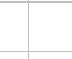
\includegraphics[max width=\textwidth]{2024_11_21_13fdaeec1d7100ca9ddcg-05(2)}
 &  &  &  &  &  &  &  &  &  &  &  &  &  &  &  &  &  &  &  &  &  &  \\
\hline
 &  &  &  &  &  &  &  &  &  &  &  &  &  &  &  &  &  &  &  &  &  &  &  &  &  &  \\
\hline
\end{tabular}
\end{center}

\section*{Zadanie 12. (0-1)}
Dla ciągu arytmetycznego \(\left(a_{n}\right)\), określonego dla \(n \geq 1\), jest spełniony warunek \(a_{4}+a_{5}+a_{6}=12\). Wtedy\\
A. \(a_{5}=4\)\\
B. \(a_{5}=3\)\\
C. \(a_{5}=6\)\\
D. \(a_{5}=5\)

\section*{Zadanie 13. (0-1)}
Dany jest ciąg geometryczny \(\left(a_{n}\right)\), określony dla \(n \geq 1\), w którym \(a_{1}=\sqrt{2}, \quad a_{2}=2 \sqrt{2}\), \(a_{3}=4 \sqrt{2}\). Wzór na \(n\)-ty wyraz tego ciągu ma postać\\
A. \(a_{n}=(\sqrt{2})^{n}\)\\
B. \(a_{n}=\frac{2^{n}}{\sqrt{2}}\)\\
C. \(a_{n}=\left(\frac{\sqrt{2}}{2}\right)^{n}\)\\
D. \(a_{n}=\frac{(\sqrt{2})^{n}}{2}\)

\section*{Zadanie 14. (0-1)}
Przyprostokątna \(L M\) trójkąta prostokątnego \(K L M\) ma długość 3, a przeciwprostokątna \(K L\) ma długość 8 (zobacz rysunek).\\
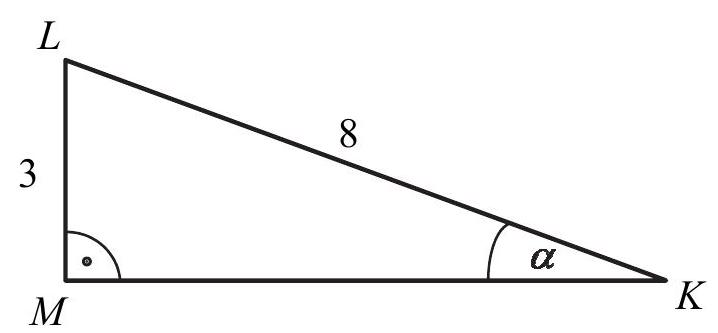
\includegraphics[max width=\textwidth, center]{2024_11_21_13fdaeec1d7100ca9ddcg-06}

Wtedy miara \(\alpha\) kąta ostrego \(L K M\) tego trójkąta spełnia warunek\\
A. \(27^{\circ}<\alpha \leq 30^{\circ}\)\\
B. \(24^{\circ}<\alpha \leq 27^{\circ}\)\\
C. \(21^{\circ}<\alpha \leq 24^{\circ}\)\\
D. \(18^{\circ}<\alpha \leq 21^{\circ}\)

\section*{Zadanie 15. (0-1)}
Dany jest trójkąt o bokach długości: \(2 \sqrt{5}, 3 \sqrt{5}, 4 \sqrt{5}\). Trójkątem podobnym do tego trójkąta jest trójkąt, którego boki mają długości\\
A. \(10,15,20\)\\
B. \(20,45,80\)\\
C. \(\sqrt{2}, \sqrt{3}, \sqrt{4}\)\\
D. \(\sqrt{5}, 2 \sqrt{5}, 3 \sqrt{5}\)

\section*{BRUDNOPIS (nie podlega ocenie)}
\begin{center}
\begin{tabular}{|c|c|c|c|c|c|c|c|c|c|c|c|c|c|c|c|c|c|c|c|c|c|c|c|c|c|c|}
\hline
 &  &  &  &  &  &  &  &  &  &  &  &  &  &  &  &  &  &  &  &  &  &  &  &  &  &  \\
\hline
 &  &  &  &  &  &  &  &  &  &  &  &  &  &  &  &  &  &  &  &  &  &  &  &  &  &  \\
\hline
 &  &  &  &  &  &  &  &  &  &  &  &  &  &  &  &  &  &  &  &  &  &  &  &  &  &  \\
\hline
 &  &  &  &  &  &  &  &  &  &  &  &  &  &  &  &  &  &  &  &  &  &  &  &  &  &  \\
\hline
 &  &  &  &  &  &  &  &  &  &  &  &  &  &  &  &  &  &  &  &  &  &  &  &  &  &  \\
\hline
 &  &  &  &  &  &  &  &  &  &  &  &  &  &  &  &  &  &  &  &  &  &  &  &  &  &  \\
\hline
 &  &  &  &  &  &  &  &  &  &  &  &  &  &  &  &  &  &  &  &  &  &  &  &  &  &  \\
\hline
 &  &  &  &  &  &  &  &  &  &  &  &  &  &  &  &  &  &  &  &  &  &  &  &  &  &  \\
\hline
 &  &  &  &  &  &  &  &  &  &  &  &  &  &  &  &  &  &  &  &  &  &  &  &  &  &  \\
\hline
 &  &  &  &  &  &  &  &  &  &  &  &  &  &  &  &  &  &  &  &  &  &  &  &  &  &  \\
\hline
 &  &  &  &  &  &  &  &  &  &  &  &  &  &  &  &  &  &  &  &  &  &  &  &  &  &  \\
\hline
 &  &  &  &  &  &  &  &  &  &  &  &  &  &  &  &  &  &  &  &  &  &  &  &  &  &  \\
\hline
 &  &  &  &  &  &  &  &  &  &  &  &  &  &  &  &  &  &  &  &  &  &  &  &  &  &  \\
\hline
 &  &  &  &  &  &  &  &  &  &  &  &  &  &  &  &  &  &  &  &  &  &  &  &  &  &  \\
\hline
 &  &  &  &  &  &  &  &  &  &  &  &  &  &  &  &  &  &  &  &  &  &  &  &  &  &  \\
\hline
 &  &  &  &  &  &  &  &  &  &  &  &  &  &  &  &  &  &  &  &  &  &  &  &  &  &  \\
\hline
 &  &  &  &  &  &  &  &  &  &  &  &  &  &  &  &  &  &  &  &  &  &  &  &  &  &  \\
\hline
 &  &  &  &  &  &  &  &  &  &  &  &  &  &  &  &  &  &  &  &  &  &  &  &  &  &  \\
\hline
 &  &  &  &  &  &  &  &  &  &  &  &  &  &  &  &  &  &  &  &  &  &  &  &  &  &  \\
\hline
 &  &  &  &  &  &  &  &  &  &  &  &  &  &  &  &  &  &  &  &  &  &  &  &  &  &  \\
\hline
 &  &  &  &  &  &  &  &  &  &  &  &  &  &  &  &  &  &  &  &  &  &  &  &  &  &  \\
\hline
 &  &  &  &  &  &  &  &  &  &  &  &  &  &  &  &  &  &  &  &  &  &  &  &  &  &  \\
\hline
 &  &  &  &  &  &  &  &  &  &  &  &  &  &  &  &  &  &  &  &  &  &  &  &  &  &  \\
\hline
 &  &  &  &  &  &  &  &  &  &  &  &  &  &  &  &  &  &  &  &  &  &  &  &  &  &  \\
\hline
 &  &  &  &  &  &  &  &  &  &  &  &  &  &  &  &  &  &  &  &  &  &  &  &  &  &  \\
\hline
 &  &  &  &  &  &  &  &  &  &  &  &  &  &  &  &  &  &  &  &  &  &  &  &  &  &  \\
\hline
 &  &  &  &  &  &  &  & 
\includegraphics[max width=\textwidth]{2024_11_21_13fdaeec1d7100ca9ddcg-07(2)}
 &  & 
\includegraphics[max width=\textwidth]{2024_11_21_13fdaeec1d7100ca9ddcg-07(1)}
 &  &  &  &  &  &  &  &  &  &  &  &  &  &  &  &  \\
\hline
 &  &  &  &  &  &  &  &  &  &  &  &  &  &  &  &  &  &  &  &  &  &  &  &  &  &  \\
\hline
 &  &  &  &  &  &  &  &  &  &  &  &  &  &  &  &  &  &  &  &  &  &  &  &  &  &  \\
\hline
 &  &  &  &  &  &  &  &  &  &  &  &  &  &  &  &  &  &  &  &  &  &  &  &  &  &  \\
\hline
 &  &  &  &  &  &  &  &  &  &  &  &  &  &  &  &  &  &  &  &  &  &  &  &  &  &  \\
\hline
 &  &  &  &  &  &  &  &  &  &  &  &  &  &  &  &  &  &  &  &  &  &  &  &  &  &  \\
\hline
 &  &  &  &  &  &  &  &  &  &  &  &  &  &  &  &  &  &  &  &  &  &  &  &  &  &  \\
\hline
 &  &  &  &  &  &  &  &  &  &  &  &  &  &  &  &  &  &  &  &  &  &  &  &  &  &  \\
\hline
 &  &  &  &  &  &  &  &  &  &  &  &  &  &  &  &  &  &  &  &  &  &  &  &  &  &  \\
\hline
 & \textbackslash  &  &  &  &  &  &  &  &  &  &  &  &  &  &  &  &  &  &  &  &  &  &  &  &  &  \\
\hline
 & - &  &  &  &  &  &  &  &  &  &  &  &  &  &  &  &  &  &  &  &  &  &  &  &  &  \\
\hline
 & - &  &  &  &  &  &  &  &  &  &  &  &  &  &  &  &  &  &  &  &  &  &  &  &  &  \\
\hline
 & \textbackslash  &  &  &  &  &  &  &  &  &  &  &  &  &  &  &  &  &  &  &  &  &  &  &  &  &  \\
\hline
 & \(\square\) &  &  &  &  &  &  &  &  &  &  &  &  &  &  &  &  &  &  &  &  &  &  &  &  &  \\
\hline
 &  &  &  &  &  &  &  &  &  &  &  &  &  &  &  &  &  &  &  &  &  &  &  &  &  &  \\
\hline
 & \textbackslash  &  &  &  &  &  &  &  &  &  &  &  &  &  &  &  &  &  &  &  &  &  &  &  &  &  \\
\hline
 &  &  &  &  &  &  &  &  &  &  &  &  &  &  &  &  &  &  &  &  &  &  &  &  &  &  \\
\hline
 &  &  &  &  &  &  &  &  &  &  &  &  &  &  &  &  &  &  &  &  &  &  &  &  &  &  \\
\hline
 & , &  &  &  &  &  &  &  &  &  &  &  &  &  &  &  &  &  &  &  &  &  &  &  &  &  \\
\hline
 &  &  &  &  &  &  &  &  &  &  &  &  &  &  &  &  &  &  &  &  &  &  &  &  &  &  \\
\hline
 &  &  &  & 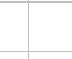
\includegraphics[max width=\textwidth]{2024_11_21_13fdaeec1d7100ca9ddcg-07}
 &  &  &  &  &  &  &  &  &  &  &  &  &  &  &  &  &  &  &  &  &  &  \\
\hline
 &  &  &  &  &  &  &  &  &  &  &  &  &  &  &  &  &  &  &  &  &  &  &  &  &  &  \\
\hline
\end{tabular}
\end{center}

\section*{Zadanie 16. (0-1)}
Dany jest okrąg o środku \(S\). Punkty \(K, L\) i \(M\) leżą na tym okręgu. Na łuku \(K L\) tego okręgu są oparte kąty \(K S L\) i \(K M L\) (zobacz rysunek), których miary \(\alpha\) i \(\beta\) spełniają warunek \(\alpha+\beta=111^{\circ}\). Wynika stąd, że\\
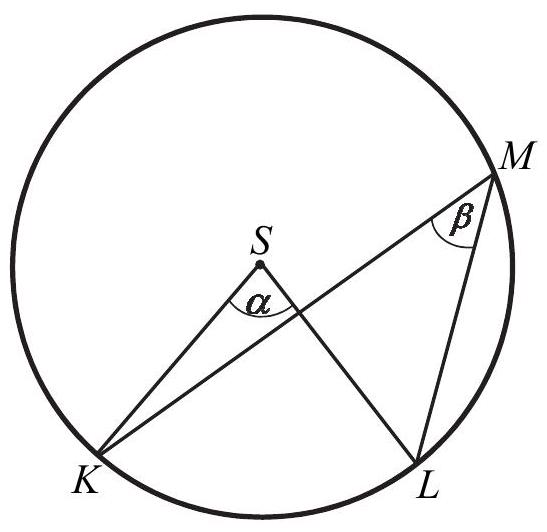
\includegraphics[max width=\textwidth, center]{2024_11_21_13fdaeec1d7100ca9ddcg-08}\\
A. \(\alpha=74^{\circ}\)\\
B. \(\alpha=76^{\circ}\)\\
C. \(\alpha=70^{\circ}\)\\
D. \(\alpha=72^{\circ}\)

\section*{Zadanie 17. (0-1)}
Dany jest trapez prostokątny \(K L M N\), którego podstawy mają długości \(|K L|=a,|M N|=b\), \(a>b\). Kąt \(K L M\) ma miarę \(60^{\circ}\). Długość ramienia \(L M\) tego trapezu jest równa\\
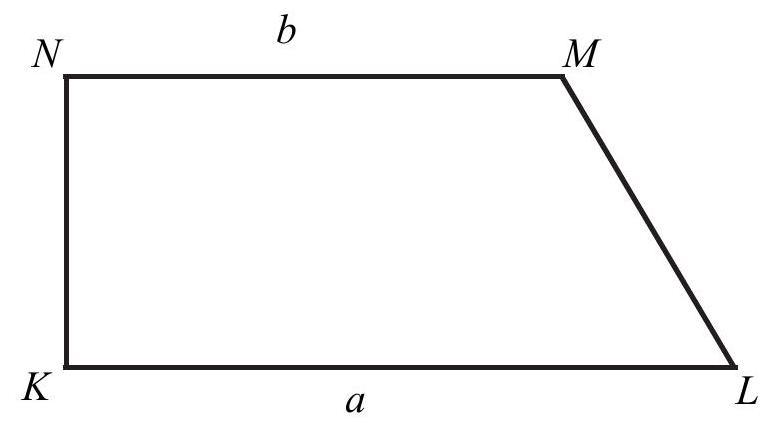
\includegraphics[max width=\textwidth, center]{2024_11_21_13fdaeec1d7100ca9ddcg-08(1)}\\
A. \(a-b\)\\
B. \(2(a-b)\)\\
C. \(a+\frac{1}{2} b\)\\
D. \(\frac{a+b}{2}\)

\section*{Zadanie 18. (0-1)}
Punkt \(K=(2,2)\) jest wierzchołkiem trójkąta równoramiennego \(K L M\), w którym \(|K M|=|L M|\). Odcinek \(M N\) jest wysokością trójkąta i \(N=(4,3)\). Zatem\\
A. \(L=(5,3)\)\\
B. \(\quad L=(6,4)\)\\
C. \(L=(3,5)\)\\
D. \(\quad L=(4,6)\)

\section*{Zadanie 19. (0-1)}
Proste o równaniach \(y=(m+2) x+3\) oraz \(y=(2 m-1) x-3\) są równoległe, gdy\\
A. \(m=2\)\\
B. \(m=3\)\\
C. \(m=0\)\\
D. \(m=1\)

\section*{BRUDNOPIS (nie podlega ocenie)}
\begin{center}

\includegraphics[max width=\textwidth]{2024_11_21_13fdaeec1d7100ca9ddcg-09}
\end{center}

\section*{Zadanie 20. (0-1)}
Podstawą ostrosłupa jest kwadrat KLMN o boku długości 4. Wysokością tego ostrosłupa jest krawędź NS, a jej długość też jest równa 4 (zobacz rysunek).\\
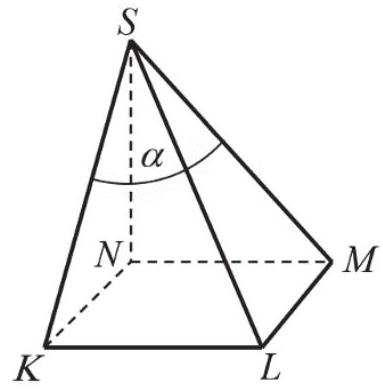
\includegraphics[max width=\textwidth, center]{2024_11_21_13fdaeec1d7100ca9ddcg-10}

Kąt \(\alpha\), jaki tworzą krawędzie \(K S\) i \(M S\), spełnia warunek\\
A. \(\alpha=45^{\circ}\)\\
B. \(45^{\circ}<\alpha<60^{\circ}\)\\
C. \(\alpha>60^{\circ}\)\\
D. \(\alpha=60^{\circ}\)

\section*{Zadanie 21. (0-1)}
Podstawą graniastosłupa prostego jest prostokąt o bokach długości 3 i 4. Kąt \(\alpha\), jaki przekątna tego graniastosłupa tworzy z jego podstawą, jest równy \(45^{\circ}\) (zobacz rysunek).\\
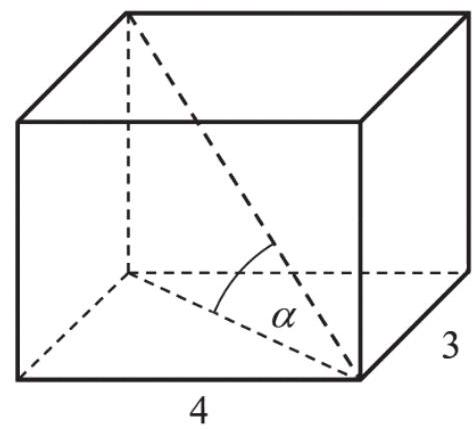
\includegraphics[max width=\textwidth, center]{2024_11_21_13fdaeec1d7100ca9ddcg-10(2)}

Wysokość graniastosłupa jest równa\\
A. 5\\
B. \(3 \sqrt{2}\)\\
C. \(5 \sqrt{2}\)\\
D. \(\frac{5 \sqrt{3}}{3}\)

\section*{Zadanie 22. (0-1)}
Na rysunku przedstawiono bryłę zbudowaną z walca i półkuli. Wysokość walca jest równa \(r\) i jest taka sama jak promień półkuli oraz taka sama jak promień podstawy walca.\\
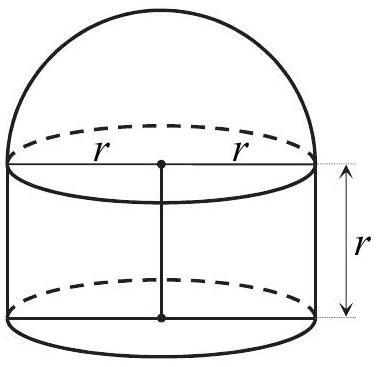
\includegraphics[max width=\textwidth, center]{2024_11_21_13fdaeec1d7100ca9ddcg-10(1)}

Objętość tej bryły jest równa\\
A. \(\frac{5}{3} \pi r^{3}\)\\
B. \(\frac{4}{3} \pi r^{3}\)\\
C. \(\frac{2}{3} \pi r^{3}\)\\
D. \(\frac{1}{3} \pi r^{3}\)

\section*{BRUDNOPIS (nie podlega ocenie)}
\begin{center}

\includegraphics[max width=\textwidth]{2024_11_21_13fdaeec1d7100ca9ddcg-11}
\end{center}

\section*{Zadanie 23. (0-1)}
W zestawie \(\underbrace{2,2,2, \ldots, 2,}_{m \text { liczb }} \underbrace{4,4,4, \ldots, 4}_{m \text { liczb }}\) jest \(2 m\) liczb \((m \geq 1)\), w tym \(m\) liczb 2 i \(m\) liczb 4.\\
Odchylenie standardowe tego zestawu liczb jest równe\\
A. 2\\
B. 1\\
C. \(\frac{1}{\sqrt{2}}\)\\
D. \(\sqrt{2}\)

\section*{Zadanie 24. (0-1)}
Ile jest wszystkich liczb naturalnych czterocyfrowych mniejszych od 2018 i podzielnych przez 5?\\
A. 402\\
B. 403\\
C. 203\\
D. 204

\section*{Zadanie 25. (0-1)}
W pudełku jest 50 kuponów, wśród których jest 15 kuponów przegrywających, a pozostałe kupony są wygrywające. Z tego pudełka w sposób losowy wyciągamy jeden kupon. Prawdopodobieństwo zdarzenia polegającego na tym, że wyciągniemy kupon wygrywający, jest równe\\
A. \(\frac{15}{35}\)\\
B. \(\frac{1}{50}\)\\
C. \(\frac{15}{50}\)\\
D. \(\frac{35}{50}\)

\section*{BRUDNOPIS (nie podlega ocenie)}
\begin{center}

\includegraphics[max width=\textwidth]{2024_11_21_13fdaeec1d7100ca9ddcg-13}
\end{center}

\section*{Zadanie 26. (0-2)}
Rozwiąż nierówność \(2 x^{2}-3 x>5\).\\

\includegraphics[max width=\textwidth, center]{2024_11_21_13fdaeec1d7100ca9ddcg-14}

Odpowiedź:

\section*{Zadanie 27. (0-2)}
Rozwiąż równanie \(\left(x^{3}+125\right)\left(x^{2}-64\right)=0\).\\

\includegraphics[max width=\textwidth, center]{2024_11_21_13fdaeec1d7100ca9ddcg-15}

Odpowiedź:

\begin{center}
\begin{tabular}{|c|l|c|c|}
\hline
\multirow{2}{*}{\begin{tabular}{l}
Wypełnia \\
egzaminator \\
\end{tabular}} & Nr zadania & 26. & 27. \\
\cline { 2 - 4 }
 & Maks. liczba pkt & 2 & 2 \\
\cline { 2 - 4 }
 & Uzyskana liczba pkt &  &  \\
\hline
\end{tabular}
\end{center}

\section*{Zadanie 28. (0-2)}
Udowodnij, że dla dowolnych liczb dodatnich \(a, b\) prawdziwa jest nierówność

\[
\frac{1}{2 a}+\frac{1}{2 b} \geq \frac{2}{a+b}
\]

\begin{center}
\begin{tabular}{|c|c|c|c|c|c|c|c|c|c|c|c|c|c|c|c|c|c|c|c|c|c|c|}
\hline
 &  &  &  &  &  &  &  &  &  &  &  &  &  &  &  &  &  &  &  &  &  &  \\
\hline
 &  &  &  &  &  &  &  &  &  &  &  &  &  &  &  &  &  &  &  &  &  &  \\
\hline
 &  &  &  &  &  &  &  &  &  &  &  &  &  &  &  &  &  &  &  &  &  &  \\
\hline
 &  &  &  &  &  &  &  &  &  &  &  &  &  &  &  &  &  &  &  &  &  &  \\
\hline
 &  &  &  &  &  &  &  &  &  &  &  &  &  &  &  &  &  &  &  &  &  &  \\
\hline
 &  &  &  &  &  &  &  &  &  &  &  &  &  &  &  &  &  &  &  &  &  &  \\
\hline
 &  &  &  &  &  &  &  &  &  &  &  &  &  &  &  &  &  &  &  &  &  &  \\
\hline
 &  &  &  &  &  &  &  &  &  &  &  &  &  &  &  &  &  &  &  &  &  &  \\
\hline
 &  &  &  &  &  &  &  &  &  &  &  &  &  &  &  &  &  &  &  &  &  &  \\
\hline
 &  &  &  &  &  &  &  &  &  &  &  &  &  &  &  &  &  &  &  &  &  &  \\
\hline
 &  &  &  &  &  &  &  &  &  &  &  &  &  &  &  &  &  &  &  &  &  &  \\
\hline
 &  &  &  &  &  &  &  &  &  &  &  &  &  &  &  &  &  &  &  &  &  &  \\
\hline
 &  &  &  &  &  &  &  &  &  &  &  &  &  &  &  &  &  &  &  &  &  &  \\
\hline
 &  &  &  &  &  &  &  &  &  &  &  &  &  &  &  &  &  &  &  &  &  &  \\
\hline
 &  &  &  &  &  &  &  &  &  &  &  &  &  &  &  &  &  &  &  &  &  &  \\
\hline
 &  &  &  &  &  &  &  &  &  &  &  &  &  &  &  &  &  &  &  &  &  &  \\
\hline
 &  &  &  &  &  &  &  &  &  &  &  &  &  &  &  &  &  &  &  &  &  &  \\
\hline
 &  &  &  &  &  &  &  &  &  &  &  &  &  &  &  &  &  &  &  &  &  &  \\
\hline
 &  &  &  &  &  &  &  &  &  &  &  &  &  &  &  &  &  &  &  &  &  &  \\
\hline
 &  &  &  &  &  &  &  &  &  &  &  &  &  &  &  &  &  &  &  &  &  &  \\
\hline
 &  &  &  &  &  &  &  &  &  &  &  &  &  &  &  &  &  &  &  &  &  &  \\
\hline
 &  &  &  &  &  &  &  &  &  &  &  &  &  &  &  &  &  &  &  &  &  &  \\
\hline
 &  &  &  &  &  &  &  &  &  &  &  &  &  &  &  &  &  &  &  &  &  &  \\
\hline
 &  &  &  &  &  &  &  &  &  &  &  &  &  &  &  &  &  &  &  &  &  &  \\
\hline
 &  &  &  &  &  &  &  &  &  &  &  &  &  &  &  &  &  &  &  &  &  &  \\
\hline
 &  &  &  &  &  &  &  &  &  &  &  &  &  &  &  &  &  &  &  &  &  &  \\
\hline
 &  &  &  &  &  &  &  &  &  &  &  &  &  &  &  &  &  &  &  &  &  &  \\
\hline
 &  &  &  &  &  &  &  &  &  &  &  &  &  &  &  &  &  &  &  &  &  &  \\
\hline
 &  &  &  &  &  &  &  &  &  &  &  &  &  &  &  &  &  &  &  &  &  &  \\
\hline
 &  &  &  &  &  &  &  &  &  &  &  &  &  &  &  &  &  &  &  &  &  &  \\
\hline
 &  &  &  &  &  &  &  &  &  &  &  &  &  &  &  &  &  &  &  &  &  &  \\
\hline
 &  &  &  &  &  &  &  &  &  &  &  &  &  &  &  &  &  &  &  &  &  &  \\
\hline
 &  &  &  &  &  &  &  &  &  &  &  &  &  &  &  &  &  &  &  &  &  &  \\
\hline
 &  &  &  &  &  &  &  &  &  &  &  &  &  &  &  &  &  &  &  &  &  &  \\
\hline
 &  &  &  &  &  &  &  &  &  &  &  &  &  &  &  &  &  &  &  &  &  &  \\
\hline
 &  &  &  &  &  &  &  &  &  &  &  &  &  &  &  &  &  &  &  &  &  &  \\
\hline
 &  &  &  &  &  &  &  &  &  &  &  &  &  &  &  &  &  &  &  &  &  &  \\
\hline
 &  &  &  &  &  &  &  &  &  &  &  &  &  &  &  &  &  &  &  &  &  &  \\
\hline
 &  &  &  &  &  &  &  &  &  &  &  &  &  &  &  &  &  &  &  &  &  &  \\
\hline
 &  &  &  &  &  &  &  &  &  &  &  &  &  &  &  &  &  &  &  &  &  &  \\
\hline
 &  &  &  &  &  &  &  &  &  &  &  &  &  &  &  &  &  &  &  &  &  &  \\
\hline
 &  &  &  &  &  &  &  &  &  &  &  &  &  &  &  &  &  &  &  &  &  &  \\
\hline
 &  &  &  &  &  &  &  &  &  &  &  &  &  &  &  &  &  &  &  &  &  &  \\
\hline
\end{tabular}
\end{center}

Zadanie 29. (0-2)\\
Okręgi o środkach odpowiednio \(A\) i \(B\) są styczne zewnętrznie i każdy z nich jest styczny do obu ramion danego kąta prostego (zobacz rysunek). Promień okręgu o środku \(A\) jest równy 2.\\
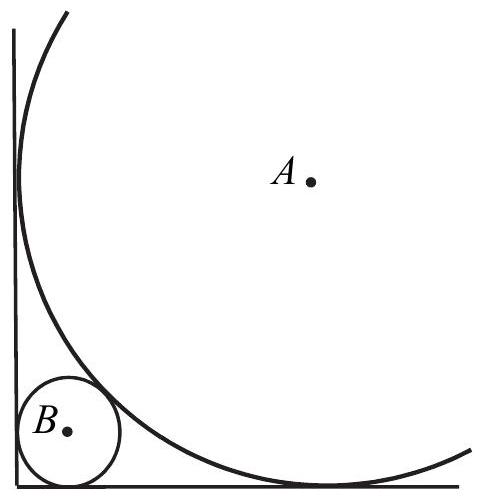
\includegraphics[max width=\textwidth, center]{2024_11_21_13fdaeec1d7100ca9ddcg-17}

Uzasadnij, że promień okręgu o środku \(B\) jest mniejszy od \(\sqrt{2}-1\).\\

\includegraphics[max width=\textwidth, center]{2024_11_21_13fdaeec1d7100ca9ddcg-17(1)}

\begin{center}
\begin{tabular}{|c|l|c|c|}
\hline
\multirow{2}{*}{\begin{tabular}{c}
Wypetnia \\
egzaminator \\
\end{tabular}} & Nr zadania & 28. & 29. \\
\cline { 2 - 4 }
 & Maks. liczba pkt & 2 & 2 \\
\cline { 2 - 4 }
 & Uzyskana liczba pkt &  &  \\
\hline
\end{tabular}
\end{center}

\section*{Zadanie 30. (0-2)}
Do wykresu funkcji wykładniczej, określonej dla każdej liczby rzeczywistej \(x\) wzorem \(f(x)=a^{x}\) (gdzie \(a>0\) i \(a \neq 1\) ), należy punkt \(P=(2,9)\). Oblicz \(a\) i zapisz zbiór wartości funkcji \(g\), określonej wzorem \(g(x)=f(x)-2\).\\

\includegraphics[max width=\textwidth, center]{2024_11_21_13fdaeec1d7100ca9ddcg-18}

Odpowiedź: \(\qquad\)

\section*{Zadanie 31. (0-2)}
Dwunasty wyraz ciągu arytmetycznego \(\left(a_{n}\right)\), określonego dla \(n \geq 1\), jest równy 30 , a suma jego dwunastu początkowych wyrazów jest równa 162 . Oblicz pierwszy wyraz tego ciągu.\\

\includegraphics[max width=\textwidth, center]{2024_11_21_13fdaeec1d7100ca9ddcg-19}

Odpowiedź: \(\qquad\)

\begin{center}
\begin{tabular}{|c|l|c|c|}
\hline
\multirow{2}{*}{\begin{tabular}{c}
Wypełnia \\
egzaminator \\
\end{tabular}} & Nr zadania & \(\mathbf{3 0 .}\) & \(\mathbf{3 1 .}\) \\
\cline { 2 - 4 }
 & Maks. liczba pkt & \(\mathbf{2}\) & \(\mathbf{2}\) \\
\cline { 2 - 4 }
 & Uzyskana liczba pkt &  &  \\
\hline
\end{tabular}
\end{center}

\section*{Zadanie 32. (0-5)}
W układzie współrzędnych punkty \(A=(4,3)\) i \(B=(10,5)\) są wierzchołkami trójkąta \(A B C\).\\
Wierzchołek \(C\) leży na prostej o równaniu \(y=2 x+3\). Oblicz współrzędne punktu \(C\), dla którego kąt \(A B C\) jest prosty.\\

\includegraphics[max width=\textwidth, center]{2024_11_21_13fdaeec1d7100ca9ddcg-20}\\

\includegraphics[max width=\textwidth, center]{2024_11_21_13fdaeec1d7100ca9ddcg-21}

Odpowiedź: \(\qquad\)

\begin{center}
\begin{tabular}{|c|l|c|}
\hline
\multirow{2}{*}{\begin{tabular}{l}
Wypelnia \\
egzaminator \\
\end{tabular}} & Nr zadania & 32. \\
\cline { 2 - 3 }
 & Maks. liczba pkt & 5 \\
\cline { 2 - 3 }
 & Uzyskana liczba pkt &  \\
\hline
\end{tabular}
\end{center}

\section*{Zadanie 33. (0-4)}
Dane są dwa zbiory: \(A=\{100,200,300,400,500,600,700\}\) i \(B=\{10,11,12,13,14,15,16\}\). Z każdego z nich losujemy jedną liczbę. Oblicz prawdopodobieństwo zdarzenia polegającego na tym, że suma wylosowanych liczb będzie podzielna przez 3. Obliczone prawdopodobieństwo zapisz w postaci nieskracalnego ułamka zwykłego.\\

\includegraphics[max width=\textwidth, center]{2024_11_21_13fdaeec1d7100ca9ddcg-22}\\

\includegraphics[max width=\textwidth, center]{2024_11_21_13fdaeec1d7100ca9ddcg-23}

Odpowiedź: \(\qquad\)

\begin{center}
\begin{tabular}{|c|l|c|}
\hline
\multirow{2}{*}{\begin{tabular}{l}
Wypelnia \\
egzaminator \\
\end{tabular}} & Nr zadania & 33. \\
\cline { 2 - 3 }
 & Maks. liczba pkt & 4 \\
\cline { 2 - 3 }
 & Uzyskana liczba pkt &  \\
\hline
\end{tabular}
\end{center}

\section*{Zadanie 34. (0-4)}
Dany jest graniastosłup prawidłowy trójkątny (zobacz rysunek). Pole powierzchni całkowitej tego graniastosłupa jest równe \(45 \sqrt{3}\). Pole podstawy graniastosłupa jest równe polu jednej ściany bocznej. Oblicz objętość tego graniastosłupa.\\

\includegraphics[max width=\textwidth, center]{2024_11_21_13fdaeec1d7100ca9ddcg-24}

\begin{center}
\begin{tabular}{|c|c|c|c|c|c|c|c|c|c|c|c|c|c|c|c|c|c|c|c|c|c|c|c|c|c|c|}
\hline
 &  &  &  &  &  &  &  &  &  &  &  &  &  &  &  &  &  &  &  &  &  &  &  &  &  &  \\
\hline
 &  &  &  &  &  &  &  &  &  &  &  &  &  &  &  &  &  &  &  &  &  &  &  &  &  &  \\
\hline
 &  &  &  &  &  &  &  &  &  &  &  &  &  &  &  &  &  &  &  &  &  &  &  &  &  &  \\
\hline
 &  &  &  &  &  &  &  &  &  &  &  &  &  &  &  &  &  &  &  &  &  &  &  &  &  &  \\
\hline
 &  &  &  &  &  &  &  &  &  &  &  &  &  &  &  &  &  &  &  &  &  &  &  &  &  &  \\
\hline
 &  &  &  &  &  &  &  &  &  &  &  &  &  &  &  &  &  &  &  &  &  &  &  &  &  &  \\
\hline
 &  &  &  &  &  &  &  &  &  &  &  &  &  &  &  &  &  &  &  &  &  &  &  &  &  &  \\
\hline
 &  &  &  &  &  &  &  &  &  &  &  &  &  &  &  &  &  &  &  &  &  &  &  &  &  &  \\
\hline
 &  &  &  &  &  &  &  &  &  &  &  &  &  &  &  &  &  &  &  &  &  &  &  &  &  &  \\
\hline
 &  &  &  &  &  &  &  &  &  &  &  &  &  &  &  &  &  &  &  &  &  &  &  &  &  &  \\
\hline
 &  &  &  &  &  &  &  &  &  &  &  &  &  &  &  &  &  &  &  &  &  &  &  &  &  &  \\
\hline
 &  &  &  &  &  &  &  &  &  &  &  &  &  &  &  &  &  &  &  &  &  &  &  &  &  &  \\
\hline
 &  &  &  &  &  &  &  &  &  &  &  &  &  &  &  &  &  &  &  &  &  &  &  &  &  &  \\
\hline
 &  &  &  &  &  &  &  &  &  &  &  &  &  &  &  &  &  &  &  &  &  &  &  &  &  &  \\
\hline
 &  &  &  &  &  &  &  &  &  &  &  &  &  &  &  &  &  &  &  &  &  &  &  &  &  &  \\
\hline
 &  &  &  &  &  &  &  &  &  &  &  &  &  &  &  &  &  &  &  &  &  &  &  &  &  &  \\
\hline
 &  &  &  &  &  &  &  &  &  &  &  &  &  &  &  &  &  &  &  &  &  &  &  &  &  &  \\
\hline
 &  &  &  &  &  &  &  &  &  &  &  &  &  &  &  &  &  &  &  &  &  &  &  &  &  &  \\
\hline
 &  &  &  &  &  &  &  &  &  &  &  &  &  &  &  &  &  &  &  &  &  &  &  &  &  &  \\
\hline
 &  &  &  &  &  &  &  &  &  &  &  &  &  &  &  &  &  &  &  &  &  &  &  &  &  &  \\
\hline
 &  &  &  &  &  &  &  &  &  &  &  &  &  &  &  &  &  &  &  &  &  &  &  &  &  &  \\
\hline
 &  &  &  &  &  &  &  &  &  &  &  &  &  &  &  &  &  &  &  &  &  &  &  &  &  &  \\
\hline
 &  &  &  &  &  &  &  &  &  &  &  &  &  &  &  &  &  &  &  &  &  &  &  &  &  &  \\
\hline
 &  &  &  &  &  &  &  &  &  &  &  &  &  &  &  &  &  &  &  &  &  &  &  &  &  &  \\
\hline
 &  &  &  &  &  &  &  &  &  &  &  &  &  &  &  &  &  &  &  &  &  &  &  &  &  &  \\
\hline
 &  &  &  &  &  &  &  &  &  &  &  &  &  &  &  &  &  &  &  &  &  &  &  &  &  &  \\
\hline
 &  &  &  &  &  &  &  &  &  &  &  &  &  &  &  &  &  &  &  &  &  &  &  &  &  &  \\
\hline
 &  &  &  &  &  &  &  &  &  &  &  &  &  &  &  &  &  &  &  &  &  &  &  &  &  &  \\
\hline
 &  &  &  &  &  &  &  &  &  &  &  &  &  &  &  &  &  &  &  &  &  &  &  &  &  &  \\
\hline
 &  &  &  &  &  &  &  &  &  &  &  &  &  &  &  &  &  &  &  &  &  &  &  &  &  &  \\
\hline
 &  &  &  &  &  &  &  &  &  &  &  &  &  &  &  &  &  &  &  &  &  &  &  &  &  &  \\
\hline
 &  &  &  &  &  &  &  &  &  &  &  &  &  &  &  &  &  &  &  &  &  &  &  &  &  &  \\
\hline
 &  &  &  &  &  &  &  &  &  &  &  &  &  &  &  &  &  &  &  &  &  &  &  &  &  &  \\
\hline
 &  &  &  &  &  &  &  &  &  &  &  &  &  &  &  &  &  &  &  &  &  &  &  &  &  &  \\
\hline
 &  &  &  &  &  &  &  &  &  &  &  &  &  &  &  &  &  &  &  &  &  &  &  &  &  &  \\
\hline
 &  &  &  &  &  &  &  &  &  &  &  &  &  &  &  &  &  &  &  &  &  &  &  &  &  &  \\
\hline
 &  &  &  &  &  &  &  &  &  &  &  &  &  &  &  &  &  &  &  &  &  &  &  &  &  &  \\
\hline
 &  &  &  &  &  &  &  &  &  &  &  &  &  &  &  &  &  &  &  &  &  &  &  &  &  &  \\
\hline
 &  &  &  &  &  &  &  &  &  &  &  &  &  &  &  &  &  &  &  &  &  &  &  &  &  &  \\
\hline
 &  &  &  &  &  &  &  &  &  &  &  &  &  &  &  &  &  &  &  &  &  &  &  &  &  &  \\
\hline
 &  &  &  &  &  &  &  &  &  &  &  &  &  &  &  &  &  &  &  &  &  &  &  &  &  &  \\
\hline
 &  &  &  &  &  &  &  &  &  &  &  &  &  &  &  &  &  &  &  &  &  &  &  &  &  &  \\
\hline
 &  &  &  &  &  &  &  &  &  &  &  &  &  &  &  &  &  &  &  &  &  &  &  &  &  &  \\
\hline
 &  &  &  &  &  &  &  &  &  &  &  &  &  &  &  &  &  &  &  &  &  &  &  &  &  &  \\
\hline
\end{tabular}
\end{center}

Odpowiedź: \(\qquad\)

\begin{center}
\begin{tabular}{|c|l|c|}
\hline
\multirow{2}{*}{\begin{tabular}{l}
Wypelnia \\
egzaminator \\
\end{tabular}} & Nr zadania & 34. \\
\cline { 2 - 3 }
 & Maks. liczba pkt & 4 \\
\cline { 2 - 3 }
 & Uzyskana liczba pkt &  \\
\hline
\end{tabular}
\end{center}

\section*{BRUDNOPIS (nie podlega ocenie)}

\end{document}